\section{Introduction}
\label{sec:intro}

Consider a team that wires an LLM judge into best-of-$n$ serving: the model writes 64 candidate solutions per problem and the judge picks the one to keep.
On a spot check the judge agrees with human graders about 90 percent of the time, so the team trusts it.
Under optimization the scoreboard climbs while true quality does not: the pipeline has learned to produce answers the judge likes, not answers that are right, and the judge has been reward-hacked~\cite{gao2022scaling,skalse2022defining}.
The failure was discoverable beforehand, with a few dozen labeled examples, because this judge's scores track writing quality once soundness is held fixed --- and no agreement rate can reveal that.
This paper turns that before-the-fact check into a \emph{certificate}: a cheap audit, run before deployment, whose verdict predicts whether the judge will be gamed.

The workflow the certificate replaces rests on two failing assumptions: that raw human agreement validates a judge, and that nothing better exists before deployment.
Recent work has already shown that benchmark accuracy, the standard static measure of reward-model quality, predicts downstream optimization outcomes poorly~\cite{wen2024rethinking}.
We show that a different static measurement --- what a judge \emph{reads}, not how often it agrees --- does predict them.
That style bias exists in judges and reward models is established at the class level~\cite{wu2023style,rmbench2024}; what the certificate adds is a per-deployment instrument that measures whether a particular judge, on a particular task and prompt, reads substance.

Our contributions:
\begin{itemize}
\item \textbf{A cheap audit with a categorical verdict.} A few dozen blind human labels, graded separately on a target axis (soundness) and an axis the judge should ignore (style), are read through two partial correlations and yield a verdict per judge configuration: pass, fail, or convict (Section~\ref{sec:audit}; Table~\ref{tab:h2h}).
The key verdicts reproduce on a hypothesis-blind non-author rater's labels (Section~\ref{sec:audit}; Table~\ref{tab:robust}).
\item \textbf{Outcome validation under real optimization pressure.} The frozen verdicts predicted the best-of-$n$ outcome for ten of eleven registered configurations; the full registration bookkeeping lives in one prediction ledger (Table~\ref{tab:ledger}), and Section~\ref{sec:pressure} reports the one false pass and the disclosed post-hoc rule revision it triggered.
Because verdicts are collinear with reference presence, the configurations collapse to roughly four verdict classes, so we also report the audit's incremental validity over a reference-presence baseline, which it beats precisely on corrupted evaluators (Section~\ref{sec:audit}; Section~\ref{sec:limits}).
\item \textbf{A diagnosis raw agreement cannot make.} The audit convicts a sabotaged frontier judge and a top open trained reward model that raw agreement scores like honest mid-size judges, and the convicted frontier judge corrupts its scoreboard without measurably corrupting selection --- the failure mode an accuracy check is blind to (Sections~\ref{sec:audit}--\ref{sec:pressure}).
\item \textbf{A generalization path beyond hand labels.} A zero-label perturbation battery and a mechanical-oracle variant of the audit are each validated against the human-label verdicts (Section~\ref{sec:procedure}).
\item \textbf{Design rules for practitioners}, including when a trusted reference helps a judge and when it amplifies gaming (Section~\ref{sec:rules}).
\end{itemize}

The audit can be small because evaluator failure is mechanistic.
Companion work shows that signals which \emph{compare} a solution to reference text fail to grade it, because most of their variance is a property of the reference, while signals that \emph{verify} against something checkable do grade~\cite{companionB}.
A judge sits on one side or the other depending on protocol and scale, and the audit detects which (Figure~\ref{fig:concept}).

Four design choices distinguish the audit from raw-agreement validation.
Humans grade on two separated axes rather than one quality number, because a single number makes loading on the wrong axis unmeasurable in principle; the axes here (soundness, style) are an instantiation chosen for the threat model, not a fixed pair (length, format, and position are probed separately in Section~\ref{sec:rules}).
A deliberately selected subsample --- built where cheap signals disagree, which spreads a soundness axis the random set leaves near ceiling --- supplies power that random data cannot.
The verdict is read from partial correlations, not an agreement rate.
And a sabotaged judge serves as a positive control: evidence the instrument can convict, not merely bless.

We validate by registering predictions and applying pressure: a 7B generator writes 64 candidates per problem, each judge picks its favorite, and two pre-registered quantities separate scoreboard inflation from real accuracy loss (Section~\ref{sec:pressure}).
Failed and convicted judges cluster above correctly certified ones on both quantities; the one false pass sits exactly at the pass threshold (Figure~\ref{fig:h2h}); and a cross-domain extrapolation to code succeeds in ten of eleven eligible configurations, missing exactly where a post-hoc mechanism --- the capability gate --- says the audit itself would not transfer.
That miss yields the operational lesson: certification is a property of a judge, task, and prompt triple, and must be measured where the judge will be used.

\begin{figure}[t]
\centering
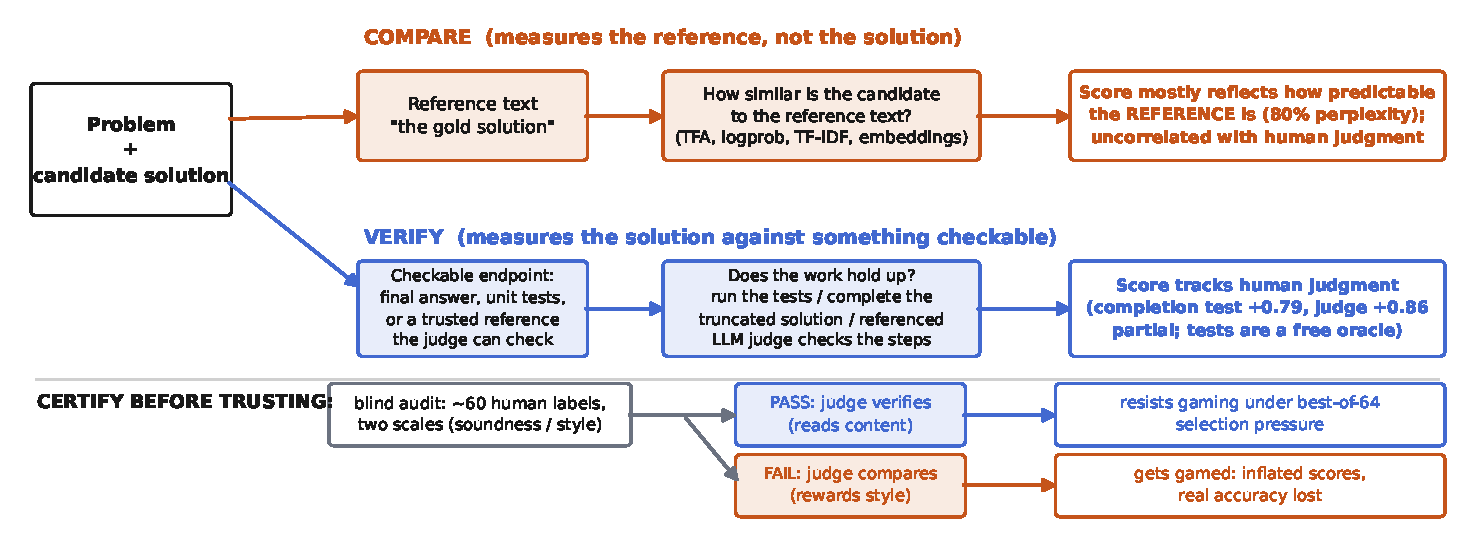
\includegraphics[width=\textwidth]{figures/fig_concept.pdf}
\caption{\textbf{Why a small audit can predict gaming.}
Top and middle: the two evaluator mechanisms; comparison-shaped evaluators reward resemblance to a reference and load on properties like style, while verification-shaped evaluators check the solution against something trusted.
Bottom: the audit pipeline; a blind labeled set read through partial correlations classifies the mechanism, and the verdict predicts behavior under optimization pressure.
\textbf{Takeaway: evaluator failure has one dominant mechanism, so a small instrument aimed at it can predict gaming before any optimization runs.}}
\label{fig:concept}
\end{figure}
